\chapter{The effect of viscosity on the Kelvin-Helmholtz instability in the fan plane of a null point}

\graphicspath{{images/null_point_khi/}}

\section{Introduction}

\subsection{Why are nulls important?}

Null points are an abundant feature in the topologically complex magnetic field of the solar corona [TODO reference to estimate of null points] and are inferred to participate in a number of high-energy phenomena. One such important phenomena is the compact solar flare, thought to arise due to energetic reconnection events occurring in the vicinity of a null, resulting in a flare with a much shorter, brighter life than those associated with coronal loops. Due to the shape of the null, these flares are typically associated with a signatory circular flare ribbon. Null points are also susceptible to collapse, a process that has been theoretically shown to potentially produce oscillatory reconnection TODO ref. The dissipation mechanisms, primarily viscosity and resistivity, can have a strong effect on the dynamic development of the null, particularly the development of reconnection in and around the null point. Aside from the importance of investigating the effect of dissipation on such energetic phenomena, the null point, due to its variation in magnetic field strength, is also an ideal test for the recently developed model of anisotropic viscosity, the switching model. TODO MENTION PRIOR TESTS

Here, we consider an idealised null point which we dynamically stress by twisting the spine. Due to the high speed at which we do this, thin shear layers in the velocity develop along the fan plane which can become unstable to the Kelvin-Helmholtz instability. The vortices created can then go on to promote reconnection in the fan plane. 

\section{Methods}

\subsection{Numerical setup}

The magnetic structure of the null point with the spine aligned along the $z$-axis is written
\begin{equation}
  \label{eq:null_point_field}
  \vec{B} = (x, y, -2z).
\end{equation}
Since we wish to dynamically stress this null point, we let the initial velocity be uniformly zero, $\vec{u} = \vec{0}$. We also set a uniform density $\rho = 1$ and internal energy $\varepsilon = TODO$, corresponding to a temperature of $T = TODO$. At the upper and lower $z$-boundaries we impose a twisting motion centred around the axis of the null with a smooth, $\tanh$-shaped radial profile which is accelerated from stationary using a $\tanh^2$-shaped ramping function. The velocity at the upper boundary is explicitly written as
\begin{equation}
  \label{eq:null_twisting_profile}
  \vec{u} = u_0 u_r(r) u_t(t) (-y, x),
\end{equation}
where $u_r$ describes the radial profile of the twisting motion in terms of the radius $r^2 = x^2 + y^2$,
\begin{equation}
  \label{eq:radial_twisting_function}
  u_r(r) = 1 + \tanh(1 - 36r^2),
\end{equation}
and $u_t(t)$ describes the imposed acceleration of the twisting motion,
\begin{equation}
  \label{eq:ramping_up_function}
  u_t(t) = \tanh^2(t/t_r).
\end{equation}
The peak velocity after the ramping time is approximately $u_0$, At the lower boundary, the flow is in the opposite direction.

The main parameter study required 18 simulations to be run in total; one per viscosity model for each of the 9 parameter choices. As a result we chose a relatively low resolution of $320$ grid points in each direction. In hindsight, the resolution could have been better balanced by using more grid points in the relatively long $x$ and $y$ directions than the relatively short $z$ direction. We could also have made use of a non-uniform grid, with higher resolution focussed near the null point. We believe this would have sped up the runtime of the simulations and provided slightly better quantitative results, particularly for the simulations using low values for the resistivity and viscosity, however the results as presented have been verified with higher resolution tests of a sample of simulations. These were performed at double the resolution of $640$ grid points per dimension. Due to the influence of unavoidable numerical diffusion (particularly numerical diffusion of the magnetic field) the lower resolution simulations showed slightly different timings, otherwise the results have converged.

\subsection{Tools of analysis}

There are three quantities useful in understanding the stability of the current-vortex sheet. Associated with the shear in velocity and magnetic field are two Mach numbers: the fast mode Mach number, related to the velocity shear, and the projected Alfv\'en Mach number, related to the magnetic shear,
\begin{equation}
  \label{eq:mach_numbers}
  M_f = \frac{\Delta v}{\sqrt{c_s^2 + c_A^2}} \quad \text{and} \quad M_A = \frac{\Delta v \sqrt{\rho}}{\Delta B},
\end{equation}
where $\Delta v$ and $\Delta B$ are the respective differences in the velocity and magnetic field over the shear layer, and $c_s$ and $v_A$ are the local sound and Alfv\'en speeds, respectively. Since the shear layer occurs in the presence of a guide field (that of the initial magnetic null point) which does not affect the linear stability of the KHI, we consider the Alfv\'en Mach number projected on to the layer TODO include diagram. The parameter describing the balance of stability between the tearing mode and the KHI in a current-vortex sheet is
\begin{equation}
  \label{eq:khi_stability_param}
  \Gamma = \frac{L_b}{L_v} M_A^{2/3}
\end{equation}
where $L_b$ and $L_v$ are the respective widths of the magnetic and velocity shear layers~\cite{einaudiResistiveInstabilitiesFlowing1986}. Again, due to the presence of the guide field, we consider $\Gamma$ projected on to the shear layer. Plotting the radial dependence of these quantities over the shear layers gives an idea of the probable stability. It should be noted that the stability analysis performed in reference~\cite{einaudiResistiveInstabilitiesFlowing1986} is under specific conditions. The presence of viscosity and the guide field in the system studied here require us to use their stability criteria as approximations.


TODO how did we calculate layer thickness, radius, peaks, etc

\section{Results}

\subsection{Evolution of a typical case}
\label{sec:null_point_khi_single_case}

We discuss initially the evolution of the pair of simulations using a resistivity of $\eta = 10^{-4}$ and viscosity $\nu = 10^{-4}$, comparing the two viscosity models. These simulations capture the main features of the null's response to the driver: the formation of a current-vortex sheet in the fan plane, the appearance of counterflows, the growth of both a Kelvin-Helmholtz instability and a fluting instability, and an eventual null collapse. This specific choice of parameters also highlights the differences between the isotropic and the switching viscosity models, mainly the suppression of the KHI in the isotropic case.

The total kinetic energy reveals the main developments in the simulations (Figure~\ref{fig:v-4r-4_kinetic_energy}). The initial acceleration of the drivers and injection of torsional Alfv\'en waves occurs between $t=0$ and $2$. After this time the effect of the viscosity models becomes apparent; the energy associated with the KHI grows only in the switching case, peaking between $t=9$ and $10$. Considering only the switching case, the instability generates vortices in the fan plane, encouraging current formation and enhanced Ohmic heating which in turn results in a drop of kinetic energy between $t=10$ and $12$ as the kinetic energy is converted to heat. The current sheets created during the instability also permit small, localised reconnection events, indicated by small peaks in the kinetic energy between $t=10$ and $12$. Over the same time period, the isotropic case remains stable. After $t=12$ a secondary instability, the fluting instability, occurs in both cases. Without the influence of the KHI the isotropic case becomes unstable to the fluting instability at a later time. In turn, the fluting instability triggers the collapse of the null, indicated by the associated spike in kinetic energy at $t=14$.

\begin{figure}[t]
  \centering
    \begin{subfigure}{0.49\textwidth}
      \includegraphics[width=\linewidth]{v-4r-4_kinetic_energy}
      \caption{Kinetic energy as a function of time for the isotropic (blue, solid line) and switching (orange, dashed line) cases using diffusion parameters $\nu=10^{-4}$ and $\eta=10^{-4}$. The switching case shows clear growth of the KHI starting from $t=2$. While the isotropic case shows no evidence of the KHI, there is evidence of an instability eventually leading to the null collapse at $t=14$.}
      \label{fig:v-4r-4_kinetic_energy}
    \end{subfigure}
    \hfill
    \begin{subfigure}{0.49\textwidth}
      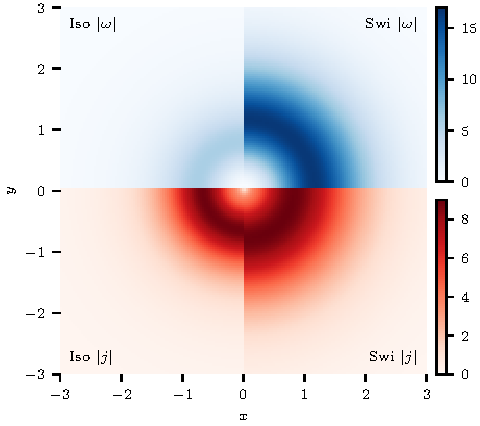
\includegraphics[width=\linewidth]{v-4r-4_vorticity_current_ring_t_3}
      \caption{Vorticity and current density rings at $t=3$. The switching model permits rings of greater radial extent and notably stronger current density.}
      \label{fig:v-4r-4_vorticity_current_ring_t_3}
    \end{subfigure}
\caption{Kinetic energy as a function of time, and the vorticity and current density rings at $t=3$.}
\label{fig:ke_and_rings}%
\end{figure}

Initially, at $t=1$ the torsional Alfv\'en waves injected by the driver trace the field surrounding the null, moving towards the fan plane and out from the spine. The waves eventually meet and create an shear layer in the velocity and magnetic field in the form of a ring of vorticity and current density. Without any diffusion in the system the main wavefronts would travel far along the field before meeting. The presence of both viscosity and resistivity encourages the waves to diffuse as they travel along the field, allowing the upper and lower waves to meet relatively close to the spine, creating rings of shear which are both thicker and smaller in radius. In the switching case, due to the switching model diffusing the field less effectively than the isotropic model, the rings are larger in radius, stronger in magnitude, and thinner (Figure~\ref{fig:v-4r-4_vorticity_current_ring_t_3}). Since the viscosity diffuses velocity directly and affects the magnetic field field indirectly, the vorticity is affected by the change in viscosity model more than the current density.

\begin{figure}[t]
  \centering
    \begin{subfigure}{0.32\textwidth}
      \includegraphics[width=\linewidth]{v-4r-4_uz_t_2}
      \caption{$t=2$}
      \label{fig:v-4r-4_uz_t_2}
    \end{subfigure}
    \begin{subfigure}{0.32\textwidth}
      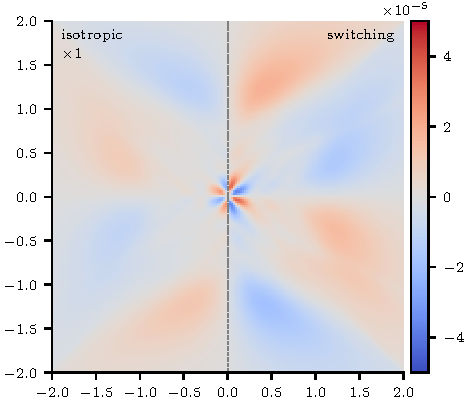
\includegraphics[width=\linewidth]{v-4r-4_uz_t_4}
      \caption{$t=4$}
      \label{fig:v-4r-4_uz_t_4}
    \end{subfigure}
    \begin{subfigure}{0.32\textwidth}
      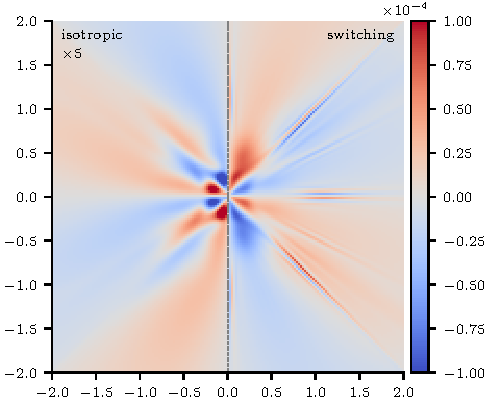
\includegraphics[width=\linewidth]{v-4r-4_uz_t_6}
      \caption{$t=6$}
      \label{fig:v-4r-4_uz_t_6}
    \end{subfigure}
    \begin{subfigure}{0.32\textwidth}
      \includegraphics[width=\linewidth]{v-4r-4_uz_t_8}
      \caption{$t=8$}
      \label{fig:v-4r-4_uz_t_8}
    \end{subfigure}
    \begin{subfigure}{0.32\textwidth}
      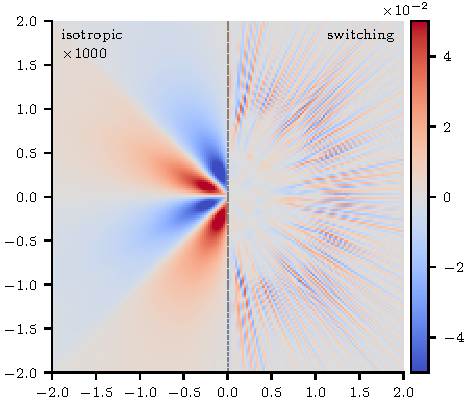
\includegraphics[width=\linewidth]{v-4r-4_uz_t_10}
      \caption{$t=10$}
      \label{fig:v-4r-4_uz_t_10}
    \end{subfigure}
    \begin{subfigure}{0.32\textwidth}
      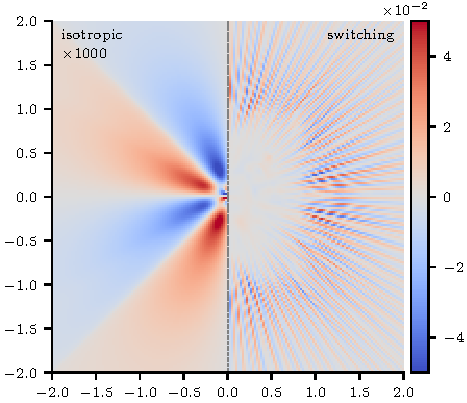
\includegraphics[width=\linewidth]{v-4r-4_uz_t_12}
      \caption{$t=12$}
      \label{fig:v-4r-4_uz_t_12}
    \end{subfigure}
\caption{Out of plane velocity at $t=2, 4, 6, 8, 10$ and $12$ for both viscosity models (isotropic on the left of each image, switching on the right). Note the isotropic results have been multiplied by as much as $1000$ in order to compare to the switching results. In the switching case an initial perturbation appears at $t=2$ and grows in amplitude as well as spreading radially, initially along the diagonals, before extending azimuthally. In the isotropic case there is no evidence of the KHI, however at $t=12$ there is evidence of what we find to be a form of fluting instability.}
\label{fig:out_of_place_velocity}%
\end{figure}

In the switching case, the velocity shear layer becomes unstable to the KHI, initially presenting as a low-amplitude perturbation overlaying the initial velocity structure. This structure appears to be associated with boundary effects (Figure~\ref{fig:v-4r-4_uz_t_2}) and is very similar comparing the two cases. The initial perturbation extends from $r\approx0.3$ to $r\approx1$. As it grows in amplitude, it spreads outwards in the fan plane, initially along the diagonals (Figure~\ref{fig:v-4r-4_uz_t_8}) before spreading azimuthally (Figure~\ref{fig:v-4r-4_uz_t_12}). The joint effect of radial spreading and perturbation growth gives rise to the specific shape of the growth in kinetic energy with time (Figure~\ref{fig:v-4r-4_kinetic_energy}). There is no evidence of the KHI in the isotropic case, however, starting from $t=8$ there is evidence of a change in behaviour very near the null, eventually creating what appear as plumes-like structures at $t=12$. As shall be discussed further on, this is the initial appearance of the fluting instability.

\begin{figure}[t]
  \centering
  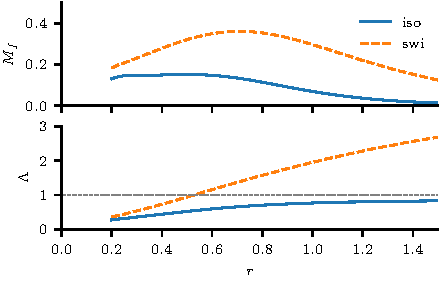
\includegraphics[width=0.5\linewidth]{v-4r-4_mach_t_6}
  \caption{Plot of the fast Mach number $M_f$ and stability measure $\Lambda$ as functions of radius $r$ at $t=6$ for the isotropic case (blue, solid line) and switching case (orange, dashed line). The measure $\Lambda$ confirms that the current-vortex sheet in the isotropic case is linearly stable to the KHI and unstable in the switching case for $r>0.5$. In the switching case the peak of $M_f$ aligns with the observed region of high growth of the instability.}%
  \label{fig:v-4r-4_mach_t_6}
\end{figure}

TODO add figure of width + magnitude of shear layers at $t=6$

Figure~\ref{fig:v-4r-4_mach_t_6} shows the relevant stability measures as functions of radius across the fan plane at $t=6$, a time where the KHI is notably unstable in the switching case and stable in the isotropic case. The stability measures show that the use of isotropic viscosity results in shear layers that are stable to the KHI, as observed. This is in contrast to the less diffusive switching viscosity which permits KHI-unstable shear layers.

\begin{figure}[t]
  \centering
    \begin{subfigure}{0.49\textwidth}
      \includegraphics[width=\linewidth]{v-4r-4_counterflows_t_3}
      \caption{Azimuthal velocity}
      \label{fig:v-4r-4_counterflows_t_3}
    \end{subfigure}
    \hfill
    \begin{subfigure}{0.49\textwidth}
      \includegraphics[width=\linewidth]{v-4r-4_lorentz_counterflows_t_3}
      \caption{Azimuthal component of Lorentz force}
      \label{fig:v-4r-4_lorentz_counterflows_t_3}
    \end{subfigure}
\caption{Azimuthal flows counter to the relevant driver are accelerated due to the action of the magnetic tension force. Both figures are sliced through $x$ and show both isotropic (left of each image) and switching (right of each image) results.}
\label{fig:counterflows}%
\end{figure}

Due to the field attempting to straighten the twist introduced by the driver, magnetic tension close to the spine opposes the direction of the twisting motion and causes counterflows to appear (Figure~\ref{fig:counterflows}). These counterflows play a part in the fluting instability found at a later time and could, with a suitable parameter choice, generate their own KHI. We do not investigate the potential for a secondary KHI further due to constraints on the numerical resolution of the simulations. This is a valid avenue of further study however, since such an instability close to the null could play a notable part in reconnection there.

\begin{figure}[t]
  \centering
    \begin{subfigure}{0.48\textwidth}
      \includegraphics[width=\linewidth]{v-4r-4_vorticity_current_ring_t_10}
      \caption{Current-vortex sheet at $t=10$ (top left is multiplied by 10)}
      \label{fig:v-4r-4_vorticity_current_ring_t_10}
    \end{subfigure}
    \hfill
    \begin{subfigure}{0.48\textwidth}
      \includegraphics[width=\linewidth]{v-4r-4_reconn_rate_t_10}
      \caption{Reconnection rate at $t=10$.}
      \label{fig:v-4r-4_reconn_rate_t_10}
    \end{subfigure}
\caption{}
\label{fig:reconnection_rate}%
\end{figure}

In both cases the current-vortex sheet grows in radius and magnitude, more in the switching case than in the isotropic, although the shearing action of the counterflows has produced a secondary ring of strong current density closer to the spine which is greater in magnitude in the isotropic case. By $t=10$ the KHI has disrupted the current-vortex sheet (Figure~\ref{fig:v-4r-4_vorticity_current_ring_t_10}) and the resultant rolls of the KHI create strong current sheets, enhancing the reconnection locally. Figure~\ref{fig:v-4r-4_reconn_rate_t_10} shows the pattern of enhanced reconnection in the switching case, visibly similar to the pattern in the current density itself, but incorporating the twist of the integrated field line.

\begin{figure}[t]
  \centering
  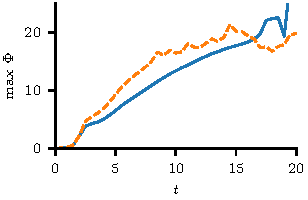
\includegraphics[width=0.5\linewidth]{v-4r-4_reconn_rate_over_time}
  \caption{Reconnection rate over time.}%
  \label{fig:v-4r-4_reconn_rate_over_time}
\end{figure}

While the enhanced reconnection in the fan plane caused by the KHI is of interest, the maximum reconnection rate actually occurs very close to the spine (Figure~\ref{fig:v-4r-4_reconn_rate_t_10}) and is notably greater in the switching case. This slippage reconnection is more efficient in the switching case due to the switching viscosity allowing much thinner, stronger current structures to evolve. Figure~\ref{fig:v-4r-4_reconn_rate_over_time} shows the peak reconnection rate in both cases as functions of time, clearly showing more efficient reconnection in the switching case.

While the Kelvin-Helmholtz instability grows in the fan plane in the switching case, both cases show growth of another instability located along the spine: the fluting instability. The competition between the inwardly directed magnetic tension in the spine, and the outwardly directed plasma pressure gradient gives rise to an interchange instability. During early stages of the instability, at around $t=6$, magnetic tension increases at four points around the centre axis. The position and number of these points are likely due to the influence of the boundaries. This perturbation in the tension is mirrored by a corresponding perturbation in the thermal pressure which acts to squeeze plasma radially outwards TODO fig of pressure, velocity and magnetic tension (or total force?). The instability continues to grow through $t=10$ with the outflows mixing with the TODO discuss dynamics of instablity after onset. 

Between $t=TODO$ and $t=TODO$ the fluting instability begins to grow (TODO this is different for switching and isotropic how?). Although this instability is influenced by the KHI and seems to influence the eventual collapse of the null, it is not a necessary component of either and so we present the relevant results here and relegate further details to chapter TODO. The instability is generated by the competition between thermal pressure and magnetic tension. 
TODO get story straight about what happens post-flute

At $t=13$ the instability appears to act as a trigger for extremely energetic reconnection in the spine, causing the numerical scheme to display artifacts in locations where the derivatives become too large. The inner

At $t=13$ the null shows some indication of beginning to reconnect and collapse, shown by the presence of velocity structures around the spine, mainly in the isotropic case. The inner ring of current density has shrunk and is now extremely strong, stronger in the isotropic case than the switching case, although we note the current structure located along the spine is around twice as strong as that around the null.

TODO finish this section.

%\begin{figure}[H]
  %\centering
  %\includegraphics[width=0.48\linewidth]{./images/null_point_khi/slices/v-4r-4-isotropic_Velocity_Vx_x_0.0_0013.pdf}
  %\includegraphics[width=0.48\linewidth]{./images/null_point_khi/slices/v-4r-4-switching_Velocity_Vx_x_0.0_0013.pdf}
%\end{figure}

%\begin{figure}[H]
  %\centering
  %\includegraphics[width=0.48\linewidth]{./images/null_point_khi/slices/v-4r-4-isotropic_magnitude_current_density_z_0.0_0013.pdf}
  %\includegraphics[width=0.48\linewidth]{./images/null_point_khi/slices/v-4r-4-switching_magnitude_current_density_z_0.0_0013.pdf}
%\end{figure}

%At $t=14$ in only the isotropic case the ring of density has shrunk entirely to the null.

%\begin{figure}[H]
  %\centering
  %\includegraphics[width=0.48\linewidth]{./images/null_point_khi/slices/v-4r-4-isotropic_magnitude_current_density_z_0.0_0014.pdf}
  %\includegraphics[width=0.48\linewidth]{./images/null_point_khi/slices/v-4r-4-switching_magnitude_current_density_z_0.0_0014.pdf}
%\end{figure}

%At this time, the reconnection rate becomes highly negative at the centre of the plot, in both cases:

%\begin{figure}[H]
  %\centering
  %\includegraphics[width=0.48\linewidth]{./images/null_point_khi/field_line_integrator/v-4r-4-isotropic_integrated_pef_0014.pdf}
  %\includegraphics[width=0.48\linewidth]{./images/null_point_khi/field_line_integrator/v-4r-4-switching_integrated_pef_0014.pdf}
%\end{figure}

%Indeed, by $t=15$, the null is showing signs of collapse in the vorticity, the velocity and in a sudden decrease in current density at the null in the isotropic case.  Note the KHI is still present and the sheer size of the vorticity in the switching case (probably due to a numerical issues, we don't have much stabalising viscous damping in this simulation). It appears as though the presence of the KHI slows the shrinking of the inner current density ring, slowing the eventual collapse of the null.

%\begin{figure}[H]
  %\centering
  %\includegraphics[width=0.48\linewidth]{./images/null_point_khi/slices/v-4r-4-isotropic_vorticity_density_z_0.0_0015.pdf}
  %\includegraphics[width=0.48\linewidth]{./images/null_point_khi/slices/v-4r-4-switching_vorticity_density_z_0.0_0015.pdf}
%\end{figure}

%\begin{figure}[H]
  %\centering
  %\includegraphics[width=0.48\linewidth]{./images/null_point_khi/slices/v-4r-4-isotropic_Velocity_Vz_z_0.0_0015.pdf}
  %\includegraphics[width=0.48\linewidth]{./images/null_point_khi/slices/v-4r-4-switching_Velocity_Vz_z_0.0_0015.pdf}
%\end{figure}

%\begin{figure}[H]
  %\centering
  %\includegraphics[width=0.48\linewidth]{./images/null_point_khi/slices/v-4r-4-isotropic_magnitude_current_density_z_0.0_0015.pdf}
  %\includegraphics[width=0.48\linewidth]{./images/null_point_khi/slices/v-4r-4-switching_magnitude_current_density_z_0.0_0015.pdf}
%\end{figure}

\subsection{Analysis of parameter study}

The results shown in section~\ref{sec:null_point_khi_single_case} do not dramatically change when the viscosity $\nu$ is varied. However, the value of $\eta$ has a strong impact on the dynamics of the stressed null. Generally, increasing $\eta$ to $10^{-3}$ produces a null that remains unstable to the KHI (when using switching viscosity) but shows no sign of collapse. In contrast, decreasing $\eta$ to $10^{-5}$ causes the null to collapse much sooner than in the example case in section~\ref{sec:null_point_khi_single_case}, so much so that the KHI doesn't have time to develop nonlinearly, even in linearly unstable cases. We present first the quantitative effect of varying $\nu$, $\eta$ and the viscosity models on the properties of the shear layers and the resulting stability and development of the KHI. We then focus our analysis on the effect of only $\eta$ on the fluting instability and the null collapse, still comparing the two viscosity models.

As an aside, in all $\nu = 10^{-3}$ isotropic simulations there's an unexpected, transient artifact in every examined variable. This was also seen in the kink instability simulations in chapter TODO. This is assumed to be due to small-amplitude fast waves created during the initial ramp up, the interaction of which causes the isotropic viscous stress tensor to produce odd effects. It appears to only affect the first time step and the effect is only to slightly increase the viscous heating. Since the affected results don't differ wildly from those of the unaffected $\nu=10{-4}$ simulations we cautiously trust these results.

\subsubsection{Properties of the shear layers and resultant instability}

We consider here the effect of varying $\nu$ and $\eta$ on the properties of the vorticity and current density rings, comparing the two viscosity models. Properties of the rings such as thickness, radial extent and peak magnitude help to give an understanding of the stability of the current-vortex sheet to the KHI. Generally, these properties vary substantially with $\eta$ for both viscosity models, substantially with $\nu$ in the isotropic cases, but only weakly with $\nu$ in the switching cases. The initial lack of dependence on $\nu$ in the switching cases is expected since the tensor is nearly zero-valued until the breakup of the current-vortex sheet, during and after which the effect of $\nu$ is much more pronounced.

\begin{figure}[h]
  \centering
  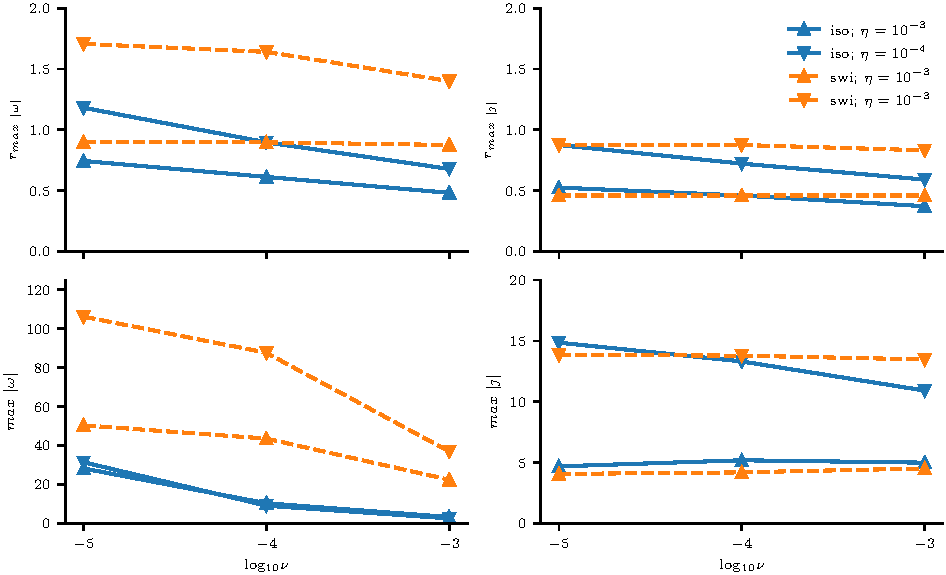
\includegraphics[width=1.0\linewidth]{param_study/peak_mag_and_loc.pdf}
  \caption{The peak magnitude within the current and vorticity rings and the radial location at which it occurs as functions of $\nu$ for each value of $\eta$. The symbols represent low resistivity (downward-facing triangle), medium resistivity (square) and high resistivity (upward-facing triangle) and the line styles represent the form of viscosity used, either isotropic (blue, solid lines) or switching (orange, dashed lines). In the isotropic case, both rings decrease in radial extent as either diffusion parameter is increased. In the switching case, both rings also decrease with $\eta$, however there is a notable increase in the radial extent with $\nu$, particularly for high values of $\eta$.}%
  \label{fig:param_study_peak_mag_and_loc}
\end{figure}

Both rings increase in radius as $\eta$ and $\nu$ decrease[TODO ref]. This is a result of the upper and lower Alfv\'en waves being able to travel further before diffusing into the fan plane and forming the shear layers. Due to the shape of the field, this allows the rings to form further from the spine in the radial direction. In the direction out of the fan plane, the thickness of both the current density and vorticity shear layers decreases with decreasing $\eta$ and $\nu$ [TODO plot of thickness over time over all params]. The respective diffusion parameter naturally affects the shear layer most associated with it, that is resistivity affecting the current density layer, and viscosity affecting the vorticity layer. The viscosity affects the peak shear in each layer similarly, with the peak magnitude in either layer increasing with decreasing $\nu$[TODO 2 plots peak velocity and magnetic shear over all params over time]. This can be attributed to the lack of diffusion at lower $\nu$ allowing the same absolute difference over the shear layer in either velocity or magnetic field to exist in a thinner sheet, resulting in a greater derivative across the layer. In contrast, a decrease in $\eta$ results in a higher peak current density, as expected via a similar argument as above, but a lower peak vorticity [TODO check this]. This can be attributed to... TODO Generally, the properties of the switching layers can be considered a limiting case of the isotropic results with $\nu$ taken to zero.

\begin{figure}[h]
  \centering
  
\includegraphics[width=0.8\linewidth]{param_study/kinetic_energies.pdf}
  \caption{Kinetic energy against time for each parameter choice. Runs using isotropic viscosity are shown as blue (solid) lines and switching viscosity as orange (dashed) lines. The distinctive energy profile of the Kelvin-Helmholtz instability is apparent in the high and medium resistivity switching cases. Reconnection causing the collapse of the null is noted by the sharp spikes in kinetic energy near the end of the medium and low resistivity simulations. There is little dependence on $\nu$ in the switching cases, barring the low resistivity cases.}%
  \label{fig:param_study_kinetic_energies}
\end{figure}

The observed stability of KHI in the fan plane is determined via inspection of the out of plane velocity for each parameter choice, summarised in table~\ref{tab:stability}. We specifically inspect the velocity at $t=8$, before the onset of other phenomena such as the null collapse. The stability and nonlinear development is also reflected in the kinetic energies~\ref{fig:param_study_kinetic_energies}. For resistivities of $\eta = 10^{-3}$ and $10^{-4}$ using the switching model, there appears in the kinetic energy a signature growth and decay shape, indicative of the KHI. A similar pattern is also seen in the single unstable isotropic case, $(\eta, \nu) = (10^{-3}, 10^{-5})$. Isotropic cases $(10^{-3}, 10^{-4})$ and $(10^{-4}, 10^{-3})$ show similar initial increases in kinetic energy, however we do not find evidence of the KHI. Prior to $t = 8$ the kinetic energies in the switching $\eta=10^{-5}$ cases appear similar to the greater resistivity, fully unstable cases, but with a more shallow gradient. At $t=8$ there is only evidence of the KHI in the $\nu=10^{-3}$ case. By inspecting these simulations at earlier times, it's clear there is an initial KHI formed around $t=2$, however this grows so slowly that other factors dominate.

\begin{table}[]
\centering
\begin{tabular}{llllll}
$\eta$    & $\nu$    & Magnetic Prandtl number $Pr = \nu/\eta$ & Isotropic Stable? & Switching Stable? &  \\
\midrule
$10^{-5}$ & $10^{-5}$ & $1$ & Stable                 & Unstable*          &  \\
$10^{-5}$ & $10^{-4}$ & $10$ & Stable                 & Unstable*          &  \\
$10^{-5}$ & $10^{-3}$ & $100$ & Stable                 & Unstable*          &  \\
$10^{-4}$ & $10^{-5}$ & $0.1$ & Stable                 & Unstable                 &  \\
$10^{-4}$ & $10^{-4}$ & $1$ & Stable                 & Unstable                 &  \\
$10^{-4}$ & $10^{-3}$ & $10$ & Stable                 & Unstable                 &  \\
$10^{-3}$ & $10^{-5}$ & $0.01$ & Unstable                 & Unstable                 &  \\
$10^{-3}$ & $10^{-4}$ & $0.1$ & Stable                 & Unstable                 &  \\
$10^{-3}$ & $10^{-3}$ & $1$ & Stable                 & Unstable                 & 
\end{tabular}
\caption{Stability in the isotopic and switching cases across varying $\eta$ and $\nu$. We only find one unstable isotropic simulation and no stable switching simulations, indicating the strong effect of the viscosity model on the stability of the KHI. The simulations marked Unstable* show evidence of only a very weak initial KHI and no obvious nonlinear growth.}
\label{tab:stability}
\end{table}

To further explore the observed stability of the KHI, we investigate how $M_f$ and $\Delta$ vary radially, and link to the stability and growth of the KHI. As an indicator of the stability of the shear layer, we plot the Mach number associated with the fast-mode $M_f = \frac{\Delta v}{\sqrt{c_s^2 + c_A^2}}$, where $\Delta v$ is the difference in velocity over the shear layer, and $c_s$ and $c_A$ are the local sound and Alfv\'en speeds, respectively, as well as the parameter $\Delta = \frac{L_B}{L_v}(M_{A, proj})^{2/3}$, where $L_B$ and $L_v$ are the widths of the respective magnetic and velocity shear layers, and $M_{A, proj}$ is the Alfv\'en velocity of the layer after removing the guide field, i.e. $M_{A, proj} = \frac{\Delta v \sqrt{\rho}}{\Delta B}$ (TODO reword this entire sentence). For the layer to be theoretically unstable to the KHI, $M_f < 2$ and $\Delta > 1$.

\begin{figure}[h]
  \centering
  
\includegraphics[width=0.45\linewidth]{param_study/mach_numbers_iso.pdf}
  \includegraphics[width=0.45\linewidth]{param_study/mach_numbers_swi.pdf}
  \caption{Plots of $M_f$ and $\Delta$ as functions of $r$ for the parameters $(\nu, \eta) = (10^{-5}, 10^{-3})$ (solid line), $(10^{-4}, 10^{-4})$ (dashed line), and $(10^{-3}, 10^{-5})$ (dotted line).}%
  \label{fig:mach_numbers}
\end{figure}

As a representative sample, we plot $M_f$ and $\Delta$ for the parameters $(\nu, \eta) = (10^{-5}, 10^{-3})$, $(10^{-4}, 10^{-4})$, and $(10^{-3}, 10^{-5})$ for both the isotropic and switching models~\ref{fig:mach_numbers}. This provides a spread of parameter choices that includes examples of stable, unstable and marginally stable simulations.

Figure~\ref{fig:mach_numbers} shows the single unstable isotropic case displaying a much higher peak in the fast Mach number near the observed location of the initial KHI, around $r=0.5$. This is in contrast to the other two cases which display much smaller peaks in the Mach number and, since $\Delta < 1$ over the entire radius shown, are theoretically stable to the KHI anyway. The switching cases show two fully unstable cases and one marginally stable case. Similar to the isotropic results, the fully unstable cases show clear, high peaks at radii where $\Delta > 1$, while the marginally stable case shows a shallow peak further from the spine at a location where $\Delta \approx 1$. Comparing the two models, the effect of the isotropic viscosity is generally to reduce both $\Delta$ and $M_f$ by increasing the width of the velocity shear layer and decreasing the magnitude of the shear across it through viscous diffusion.

\subsubsection{Reconnection in the KHI}

We now consider the differences in only the switching cases, to investigate the effect of $\nu$ and $\eta$ specifically on the nonlinear development of the KHI. Before the onset the variation in the shear layer properties with $\nu$ are negligible. Generally, the main effects of different values of $\nu$ appear during the nonlinear development of the KHI, around the time $t=9$. After this time, the peaks of both current density and vorticity decrease with decreasing $\nu$ [TODO is this right and if it is why?]. [TODO how to show peaks of current density and vorticity? Another plot of peaks after $t=9$?] As seen in the example case of section~\ref{sec:null_point_khi_single_case} we find evidence of the KHI promoting slippage reconnection for $\eta = 10^{-3}$ and $10^{-4}$, the two values of $\eta$ that allow the KHI TODO plot of rolls in parallel elec field. Where $\eta=10^{-3}$, the reconnection rate varies little with $\nu$, however the rate increases with decreasing $\nu$ where $\eta=10^{-4}$, caused by TODO WHAT. Alongside the sedate, slippage reconnection, we also find evidence of bursty reconnection in the current density for these value of $\eta$ TODO plot, at $t=TODO$ for $\eta=10^{-3}$ and at the later time of $t=11$ for $\eta=10^{-4}$. Since these current structures are close to grid scale, the accuracy of these results should be viewed with caution, but they are an indicator of the potential for the KHI to promote localised, energetic reconnection events. Both slippage and bursty reconnection is evident in the single KHI-unstable isotropic case, where $\nu=10^{-5}$ and $\eta=10^{-3}$.

\subsubsection{The fluting instability}

TODO what is the behaviour of the fluting instability in all cases?

\subsubsection{The collapse of the null}

TODO For which parameters does the null collapse and what does the reconnection look like?

For $\eta=10^{-5}$, the reconnection rate is generally higher than the $10^{-4}$ simulations, particularly along the field lines that intersect the vorticity-current density ring, and along the spine until a reconnection event occurs around $t=10$ in the isotropic cases. The strength of the resultant outflows depend strongly on $\nu$, as does the proceeding reconnection within the rest of the structure, the rate of which is generally higher for weaker viscosity. In the switching case, the initial reconnection event appears sooner and, while the reconnection rate remains relatively constant across the range of $\nu$, lower viscosity does lead to a more violent resultant behaviour.

\subsection{The effect of driving velocity}

TODO
